\chapter{Introduction}

\section{PRIP Laboratory}

\subsection{Presentation}

The Pattern Recognition and Image Processing Laboratory (PRIP) is a research
group of the Vienna University of Technology (TU Wien) and is part of the
Computer Science department. The TU Wien is Austria's largest research and 
educational institution in the field of technology and natural sciences.
The Computer Science department is one of Europe's leading research and innovation 
institutions. PRIP Laboratory is focused on advanced image representations and methods 
that allow the structure of the image to become an essential part of recognition systems.
Among the people working in the PRIP Laboratory are:

\begin{itemize}
    \item Prof. Walter G. Kropatsch, Head of the Group.
    \item Dr. Jiří Hladůvka, My tutor.
    \item Majid Banaeyan, PhD student.
    \item Darshan Batavia, PhD student.
\end{itemize}

\subsection{\textit{Water's gateway to heaven} project}

\textit{Water's gateway to heaven} is an interdisciplinary research project funded 
through the Life Sciences programme on Multimodal Imaging of the Vienna Science and 
Technology Fund (WWTF) \cite{WWTF}. The project is a collaboration between three viennese 
universities: 

\begin{itemize}
    \item Plant ecophysiologists and anatomists at the University of Natural Resources 
    and Life Sciences \cite{BOKU}.
    \item Plant cell biologists at the University of Vienna \cite{UVI}.
    \item Computer scientists expert in pattern recognition and image analysis at the 
    Vienna University of Technology (TU Wien) \cite{TUV}.
\end{itemize}
%
The project focusses on the stomata, tiny pores on the surface of plant leaves. 
Stomata open and close to provide $\mathrm{CO_2}$ for photosynthesis and to limit 
water loss. This project uses novel temporal $3D$ imaging to provide a better description 
of stomatal movements in order to get a mechanistic understanding of how transient 
this movement. The goal is to answer long-standing questions about stomatal movements 
and to generate basic knowledge on how to improve stomatal responses under dynamic 
environments in order to increase net productivity and water-use efficiency \cite{WGH}.
         
\section{Technical overview}

The images use for this project are $3D$ images of leaves coming from high-resolution 
X-ray micro-tomography (micro-CT) and fluorescence microscopy. The size of the images is
$2000 \times 2000 \times 2000$ pixels. In order to track the change of the individual 
cells over time, hierarchies of abstract topological cell complexes are used, which will
reduce the image data to a neighboring structure of the plant cells without losing the
relation to the original data. This makes it possible to verify hypotheses at any time
that arise during the course of the biological analysis but may not have been known at
the time the hierarchy was built. Furthermore, this structure of the plant cells is to be
used to simulate dynamic processes \cite{PWGH}.

\subsection{Generalized maps}

The data structure chosen for this project is the $n$-dimensional generalized map
($n$-Gmap). An $n$-Gmap is a combinatorial data structure allowing to describe an
$n$-dimensional orientable or nonorientable quasi-manifold with or without boundary
\cite{Lienhardt}. This data structure is defined by a set of darts $D$ on which act
$n+1$ involutions $\alpha_i$ satisfying composition constraints of the following
definition \cite{Damiand}:

\begin{definition}[$n$-Gmap]
    An $n$-Gmap with $0<n$, is an $(n+2)$-tuple $G=(D,\alpha_0,\ldots,\alpha_{n})$ where:
    \begin{enumerate}
        \item $D$ is a finite set of darts;
        \item $\forall i\in\{0,\ldots,n\}:\alpha_i$ is an involution on $D$;
        \item $\forall i\in\{0,\ldots,n-2\},\forall j\in\{i+2,\ldots,n\}:
        \alpha_i \circ \alpha_j$ is an involution on $D$.
    \end{enumerate}
    \label{definition:gmap}
\end{definition}

\subsubsection{Python implementation}

For the project, PRIP has provided an implementation in Python based on the algorithms 
described in \cite{Lienhardt}. It consists in a hierarchy of classes which have their
root in the \textit{nGmap} class, that is an array based implementation of the
gmap, where a set of arrays is used to store the involutions. The \textit{PixelMap} class 
extends \textit{nGmap} and is a 2-Gmap representing an RxC image grid. The 
\textit{LabelMap} class extends \textit{PixelMap} and adds the possibility to build a 
2-Gmap representing an RxC image grid from a list of labels. This last class is very
useful for the project because it allows to convert the micro-CT images into a 2-Gmap
with the labels of the different leaf cells. After that we can easily make operations
on this 2-Gmap and apply image processing algorithms on it.

\subsection{Geodesic Distance Transform}

The Geodesic Distance Transform (GDT) computes distances within the connected
component of interest in a labeled image. The objects of interest are considered as
the foreground objects and the remaining objects are considered as background.
The computation of the GDT in a Gmap can be done in parallel with a logarithmic
time complexity \cite{Banaeyan}. We can compute the GDT on a labeled leaf image
to know the distance between the stomata and the mesophyll cells where the 
photosynthesis takes place. The stomata act as gates to control the amount of
$\mathrm{CO_2}$ that is released. The $\mathrm{CO_2}$ propagates through the
airspace to reach the mesophyll cells. On the figure (\ref{fig:gdt}) we inialized
the seed label as the stomata connected component and we computed the GDT
on the airspace propagation label and mesophyll cells as the target label.

\begin{figure}[ht]
    \centering
    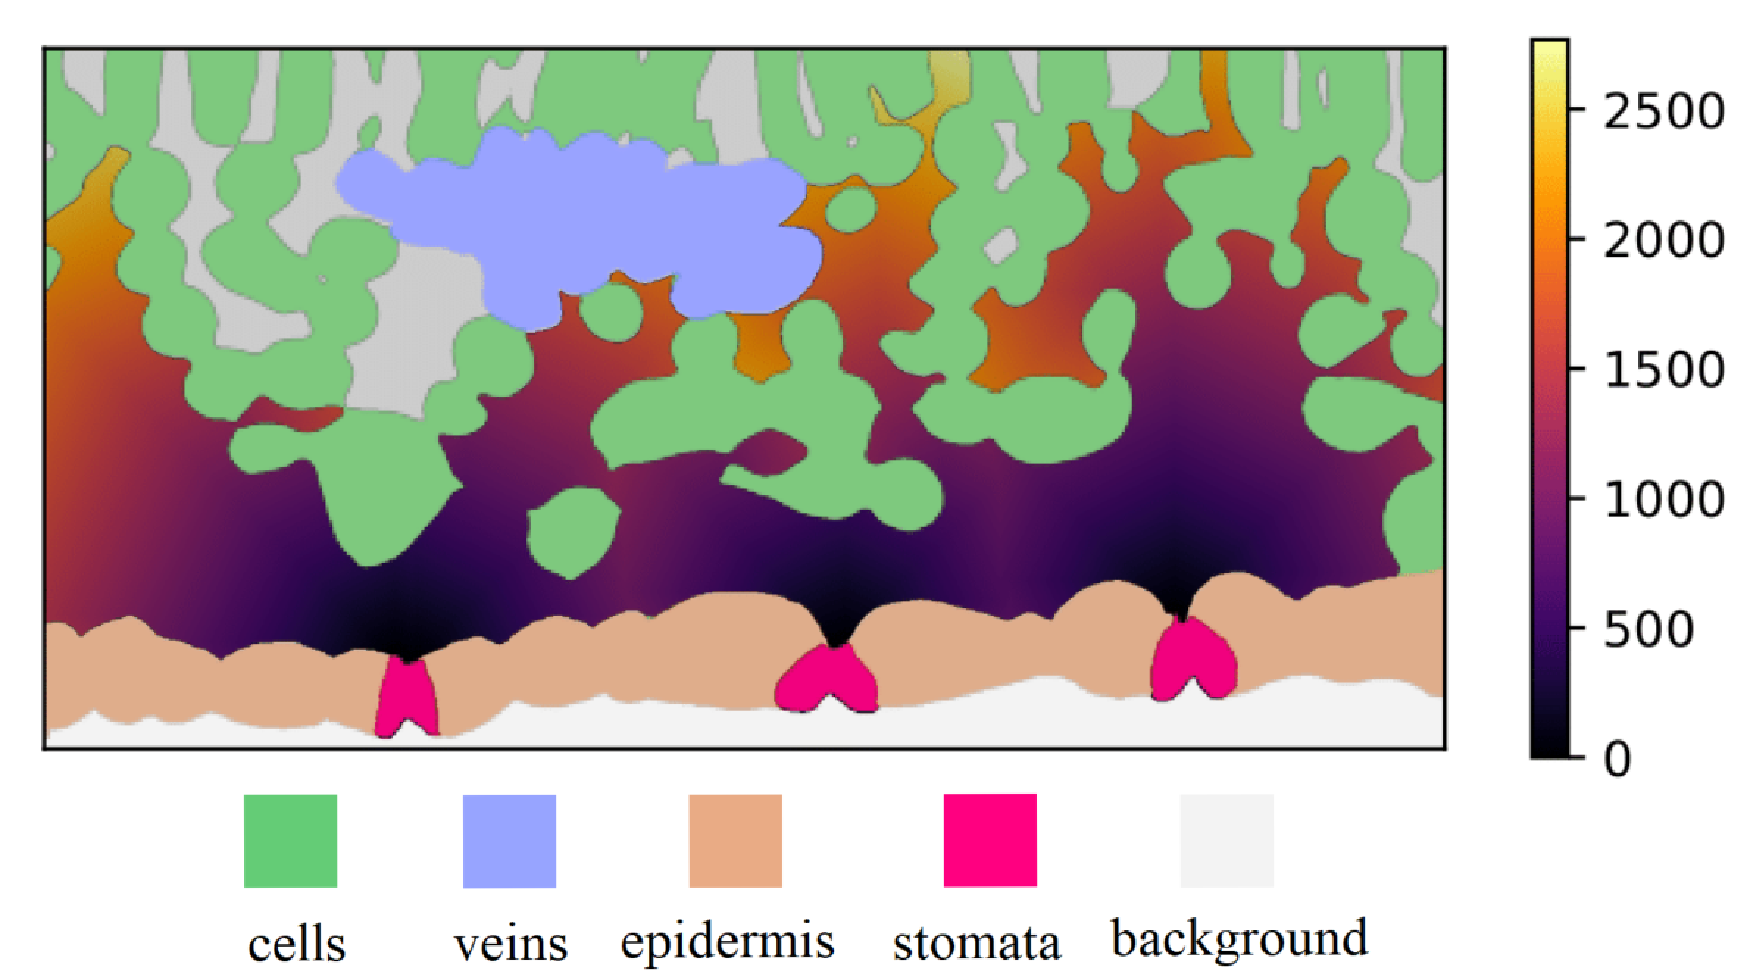
\includegraphics[width=0.8\textwidth]{figures/dt_color.pdf}
    \caption{GDT from stomata to mesophyll cells through the airspace}
    \label{fig:gdt}
\end{figure}

